\section{Diagramas de ciclos de refrigeración}\label{sec:1}

	En esta sección se utiliza como fuente principal el libro \emph{Principios de Refrigeración} de \cite[Capítulos 6 y 7]{dossat2004refrigeracion}.
	
	Los diagramas que con frecuencia se usan en el análisis del ciclo de refrigeración son los de \textit{presión-entalpia (ph)} y \textit{temperatura-entropía (Ts)}.
	
	%	Agregar gráfica de los diagramas ph y Ts para mostrar las regiones
	
	\subsection{Ciclo de refrigeración teórico} \label{sec:ciclo-teorico}
	
	%	Desarrollo del diagrama para un ciclo teórico
	
		El ciclo teórico es un ciclo de refrigeración saturado simple en el cual se supone que el vapor refrigerante que sale del evaporador y entra al compresor es vapor saturado a la temperatura y presión vaporizante, y el líquido refrigerante que sale del condensador y llega a la válvula de expansión es un líquido saturado a la temperatura y presión condensante. Además, se desprecian las pérdidas en las tuberías y en los accesorios.

		% Mencionar la disposición de los elementos y agregar la fig 7-5 del libro
		
		\begin{figure}[h]
			\centering
			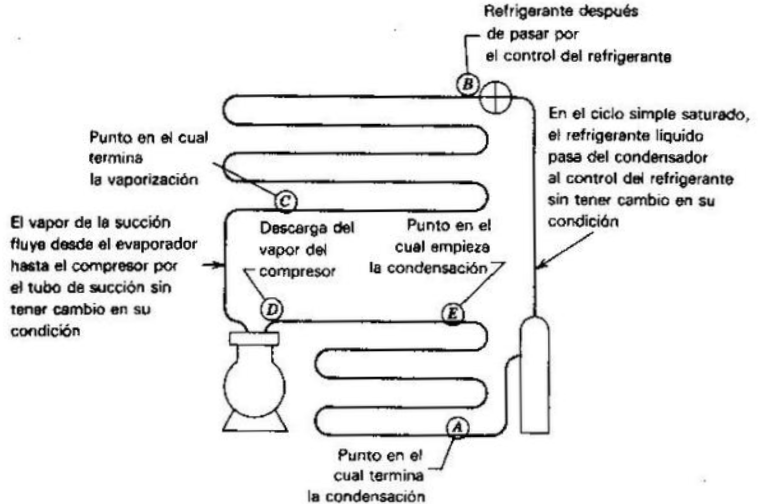
\includegraphics[width=.7\linewidth]{ciclo-saturado-simple}
			\caption{Diagrama de flujo de un ciclo saturado simple.}
			\label{fig:ciclo-teorico}
		\end{figure}
		
		\begin{figure}[h]
			\centering
			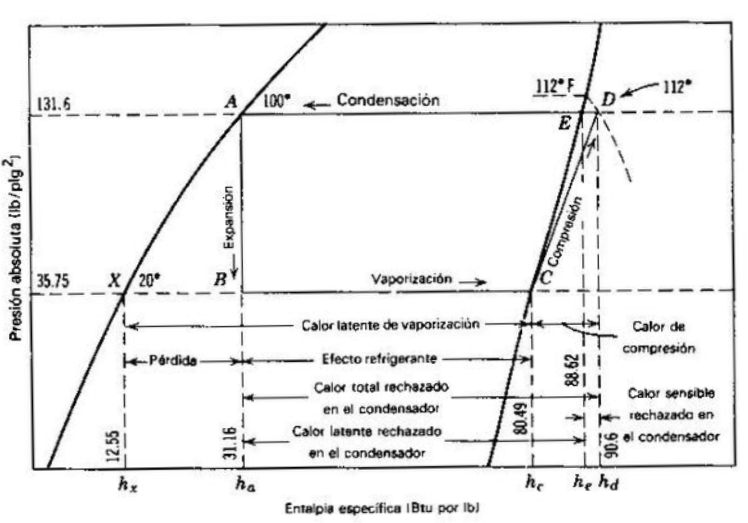
\includegraphics[width=.7\linewidth]{diagrama-ciclo-saturado-simple}
			\caption{Diagrama de flujo de un ciclo saturado simple.}
			\label{fig:diagrama-teorico}
		\end{figure}
		
		En el diagrama de la \autoref{fig:ciclo-teorico} se tiene el trazo de un ciclo saturado simple, y en la \autoref{fig:diagrama-teorico} se muestra un diagrama presión-entalpía de dicho ciclo, en el cual se observan cuatro transformaciones o procesos:
		
		\begin{itemize}
			\item Expansión.
			\item Evaporación.
			\item Compresión.
			\item Expansión.
		\end{itemize}
		
		\subsubsection{Proceso de expansión} El proceso de expansión es representado en el diagrama por el trazo $A-B$. Es un estrangulamiento tipo expansión adiabática y sucede en la válvula de expansión cuando la presión del líquido refrigerante es reducida desde la presión en el condensador a la presión en el evaporador. La temperatura del líquido que llega a la válvula de expansión A siempre es bastante mayor que la temperatura en el evaporador B y ésta deberá primero reducirse hasta dicha temperatura antes de que el líquido pueda vaporizarse en el evaporador.
			
			
			 
			En este ciclo teórico no hay ningún cambio en las propiedades del líquido refrigerante a medida que éste fluye a través de la línea de líquido desde el condensador a la válvula de expansión, y es la condición que se tiene en el punto A en el diagrama. 
			
				
				
			En este proceso, cuando el refrigerante que está a la temperatura y presión del punto A, pasa a través de la válvula de expansión, su presión se reduce a la presión del evaporador, y debe ceder suficiente calor para enfriarse a sí mismo desde la temperatura en A hasta la temperatura en B. Debido a que esta caída de presión ocurre instantáneamente, no se tiene tiempo para que tenga lugar una transferencia de calor entre el refrigerante y los alrededores. En consecuencia, el proceso es adiabático, y la disminución necesaria de temperatura del fluido se logra sólo por la transferencia de energía que se tiene dentro del fluido. Por esta razón, una parte de la masa líquida se cambia de inmediato a la fase de vapor, que se denomina \emph{vapor flash}. Esta parte que se vaporiza no produce enfriamiento útil y por lo mismo representa una pérdida de \emph{efecto refrigerante} en comparación con la suposición de que toda la masa fuera vaporizada en el evaporador.
			
			
			\subsubsection{Proceso vaporizante} El proceso $B-C$ se efectúa a presión y temperatura constantes y es la vaporización del refrigerante en el evaporador. 
			
			A medida que el refrigerante fluye a través del evaporador, este absorbe el calor del medio a refrigerar e incrementa su entalpía hasta el punto C donde estará completamente vaporizado, y es un vapor saturado a la temperatura y presión del evaporador.
			
			La distancia entre los puntos X y C en el diagrama \textit{ph} representa el calor latente total de vaporización. Entonces, ya que la distancia $B-C$ representa el efecto refrigerante, la distancia $X-B$ es la pérdida de efecto refrigerante.
				    
			\subsubsection{Proceso de compresión} En el ciclo teórico, se supone que el refrigerante mantiene sus propiedades a medida que atraviesa la línea de succión. El proceso $C-D$ se efectúa en el compresor a medida que el refrigerante incrementa su presión desde la presión del evaporador a la del condensador.
			
			En este proceso, no hay cambio en la entropía del refrigerante, por lo que, al alcanzar la presión del condensador, se encuentra en estado de vapor sobrecalentado.
				  
			\subsubsection{Proceso de condensación} El proceso $D-E$ toma lugar en una parte de la línea de descarga y en la parte superior del condensador. Esto representa el enfriamiento del vapor sobrecalentado hasta la temperatura condensante. Durante este proceso, la presión se mantiene constante. En el punto E, el refrigerante es un vapor saturado a la temperatura y presión condensante, o del condensador.
			
			El proceso $E-A$ es la condensación del vapor en el condensador y representa el calor cedido al medio exterior. 
			
			Al llegar al punto A, el refrigerante se encuentra como líquido saturado y ha completado un ciclo. Entonces, el calor total cedido por el refrigerante debe ser exactamente igual al calor absorbido en todos los demás puntos del ciclo. Por lo tanto,
			
			\begin{equation*}
				q_c = q_e + q_w
			\end{equation*}
			
			donde
			\begin{itemize}
				\item $q_c$ es el calor eliminado en el condensador,
				\item $q_e$ es el calor absorbido en el evaporador,
				\item $q_w$ es el calor absorbido equivalente debido al trabajo mecánico del compresor.
			\end{itemize}
			
	
	\subsection{Efecto de la temperatura en la eficiencia del ciclo}
	
		La eficiencia del ciclo de refrigeración compresión-vapor varía considerablemente tanto con la temperatura vaporizante como con la condensante\footnote{También se podría hacer referencia a la presión, debido a que para valores por debajo de la curva de saturación, la presión y temperatura se encuentran sobre la misma recta y permanecen constantes.}, siendo la temperatura del evaporador la que produce mayor efecto.
		
		\subsubsection{Efecto de la temperatura de succión}
		
		Si la temperatura condensante se mantiene constante, la eficiencia del ciclo disminuye al reducirse la temperatura vaporizante o de succión.\\
		
		
		Para mostrar el efecto que la temperatura de succión tiene sobre la eficiencia del ciclo, en la \autoref{fig:efecto-t-evaporador} se tienen los diagramas \emph{ph} de dos ciclos saturados simples trabajando a distintas temperaturas.
		
		\begin{figure}[h]
			\centering
			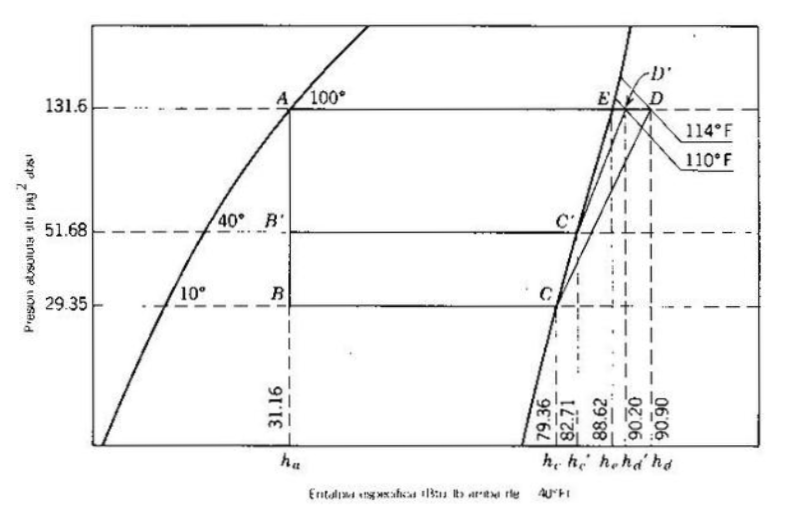
\includegraphics[width=.95\linewidth]{efecto-t-evaporador}
			\caption{Comparación entre dos ciclos saturados simples que trabajan a diferentes temperaturas vaporizantes.}
			\label{fig:efecto-t-evaporador}
		\end{figure}
		
		Uno de los dos ciclos identificados por los puntos A, B, C, D y E, el evaporador está trabajando a una temperatura de $10$ °F y el condensador a una temperatura de $100$ °F, y en los puntos A, B', C', D', y E, se tiene un ciclo similar que tiene la misma temperatura condensante pero que está trabajando a una temperatura vaporizante de $40$ °F.
		
%		Al comparar los dos ciclos se observa que el efecto refrigerante por unidad de masa es mayor para el ciclo que tiene mayor temperatura, esto debido a que se tiene un diferencial menor de temperatura entre la temperatura de baja y de alta.
		Al comparar los dos ciclos se observa que el efecto refrigerante por unidad de masa es mayor para el ciclo que tiene mayor temperatura de vaporización. Este hecho se debe a que el fluido debe ceder menos cantidad de calor para enfriarse a sí mismo a la temperatura del evaporador (proceso expuesto en la  \autoref{sec:ciclo-teorico}). \\
		
		
		\textit{En resumen, a mayor diferencial de temperatura o presión entre el condensador y el evaporador, menor será el efecto refrigerante por unidad de masa.}\\
		
		
		Por otro lado, el trabajo de compresión por unidad de masa necesario para comprimir al vapor desde la presión vaporizante hasta la presión condensante es menor para el ciclo de menor diferencial de temperatura.
		
		De manera similar, cuanto mayor sea el valor de caída de temperatura (o presión), mayor será el volumen específico y por tanto, menor será el desplazamiento volumétrico del compresor (la masa de refrigerante circulado por un compresor será menor)\footnote{En otras palabras, por cada kilogramo de refrigerante en circulación, el compresor deberá comprimir un volumen mayor de vapor.}.
		
		
		Cabe destacar que el aumento en porcentaje del volumen comprimido es mucho mayor que el aumento en porcentaje del caudal másico, lo cual, es probable que esto sea uno de los factores más importantes que influyen en la capacidad y eficiencia de un sistema de refrigeración y por consiguiente sea el más observado. Siguiendo el ejemplo expuesto en el libro (\cite[páginas 137 a 140]{dossat2004refrigeracion}), se observa que el aumento en masa es del $6.5\%$, mientras que el aumento en volumen es de $45\%$.
		
	
		\subsubsection{Efecto de la temperatura de descarga}
		
		En general, si la temperatura vaporizante se mantiene constante, disminuirá la eficiencia del ciclo al aumentarse la temperatura condensante.
		
		
		Para mostrar el efecto de la temperatura condensante sobre la eficiencia del ciclo, en la \autoref{fig:efecto-t-condensador} se muestra un diagrama \emph{ph} de dos ciclos diferentes. El ciclo A, B, C, D y E, es el cual tiene una temperatura condensante de $100$ °F, mientras que el ciclo A', B', C, D' y E', trabaja a $120$ °F.
		
		\begin{figure}[H]
			\centering
			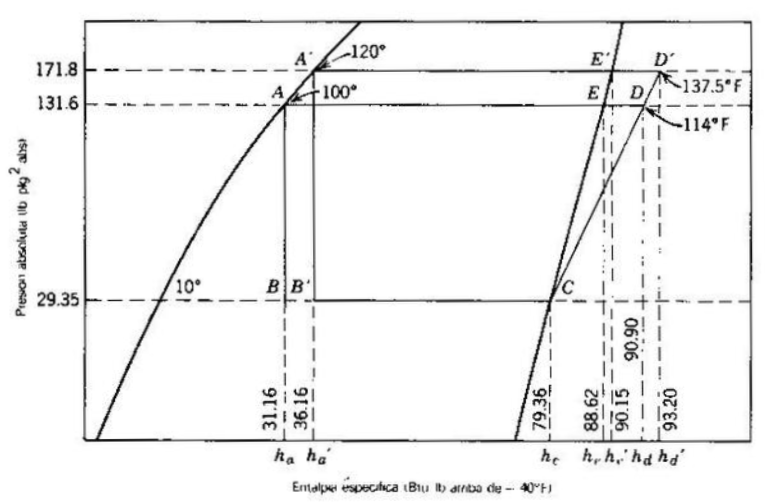
\includegraphics[width=.9\linewidth]{efecto-t-condensador}
			\caption{Comparación entre dos ciclos saturados simples que trabajan a diferentes temperaturas condensantes.}
			\label{fig:efecto-t-condensador}
		\end{figure}
		
		A medida que se aumenta la temperatura condensante, se aumenta también la temperatura que llega a la válvula de expansión y se reduce el valor del efecto refrigerante. En consecuencia, el caudal de masa del refrigerante será mayor.
		
		
		Ya que el caudal de masa es mayor para la temperatura condensante más alta, se deduce que el volumen de vapor comprimido es también mayor. Realizando un análisis, se puede observar que el aumento en porcentaje en el volumen de vapor manejado por el compresor es exactamente igual al porcentaje de aumento del caudal másico. Esto contrasta con lo que sucede cuando es variada la temperatura vaporizante.
		
		% 
		Por otro lado, debido a que la diferencia entre las presiones es grande, el trabajo de compresión por unidad de masa será mayor para el ciclo que tenga la mayor temperatura condensante. Como resultado de esto, la potencia teórica requerida también aumentará.
		
		
	\subsection{Ciclo de refrigeración real}
	
	Capítulo 9 del libro
	
		En los ciclos reales de refrigeración se tienen en cuenta ciertas consideraciones que no se contemplaron en el ciclo teórico, como la caída de presión que experimenta el fluido al paso por tuberías, evaporador, condensador, etc. Además, se considerará el subenfriamiento del líquido y el sobrecalentamiento del vapor en la tubería de succión.
		
		
		Los efectos que fueron despreciables en el ciclo teórico, y por tanto los que se considerarán en el ciclo real de refrigeración se enlistan a continuación:
		\begin{itemize}
			\item Sobrecalentamiento en el vapor de succión
			% 8-3 Sobrecalentamiento sin aprovechamiento del enfriamiento
			% 8-4 Sobrecalentamiento con aprovechamiento del enfriamiento
			% 8-5 Sobrecalentamiento en la tubería de succión (sí o sí es no aprovechado, debe aislarse la tubería): explicación de la generación de escarcha
			% 8-6 Sobrecalentamiento del vapor en el espacio refrigerado. Acá menciona la "tubería secadora"
			\item Subenfriamiento en el líquido
			% 8-7 Subenfriamiento en el líquido. Con subenfriador, o torre de enfriamiento
			% 8-8 Intercambiadores de calor. Se utilizan para subenfriar el líquido antes de la válvula de expansión. Ya que es inevitable el sobrecalentamiento del vapor de la succión en un ciclo real, sea que se uso o no un intercambiador de calor, vale la pena cualquier medio práctico que se emplee para aprovechar el enfriamiento del líquido que se tiene en el sobrecalentamiento del vapor.
			\item Pérdidas de fricción
			% 8-9 Pérdidas debidas a la fricción, en tuberías y en válvulas. Para cualquiera caso, en el lado de descarga del compresor la pérdida resulta en un aumento (inevitable) de presión y en el lado de succión, una disminución. En el resto de elementos siempre es una caída de presión. Ver diagrama
			
			
		\end{itemize}